%!TEX root = ../TaxationPlan.tex

In the previous two models discussed there was no uncertainty about what future margin would be.
Obviously in practice, there is significant uncertainty about how margin will evolve and this
uncertainty will have implications for token prices and other model outcomes. We add
uncertainty to this model by assuming that margin evolves according to a stochastic Markov process.

One additional difference we introduce in this section is a separation between the amount of fees
collected, $F_t$, and the size of the buyback, $X_t$. In the deterministic model, there were no
unexpected fluctuations and margin was either constant or always growing. These two features made it
unnecessary to store a portion of the fees collected today to fund future buybacks.

We assume that margin follows a Markov process, that is, that tomorrow's margin only depends on what
margin was today.

$$M_{t+1} = f(M_t, \varepsilon_{t+1})$$

A first order Markov process can be quite general and the margin processes from
Section~\ref{sec:dss}  and Section~\ref{sec:dg} are special cases of the above process. The only
difference is that now, margin will begin low and then will (potentially) grow to higher levels with
some uncertainty about the path it takes to get there.

Our objective will be to choose $\{X_t(M^t), F_t(M^t)\}_{t=0}^{\infty}$ to optimize certain goals.
In this document, we will focus on minimizing the present discounted value of payouts to token
holders and keeping fee rates at a low and consistent level\footnote{We do this by using a quadratic
punishment function which punishes any deviation of the fee rate from 0 quadratically. The quadratic
structure ensures that large fees are penalized more heavily than smaller fees --- Under certain
assumptions, such a structure often produces a solution in which fees tomorrow are the same as the
fees today in expectation}.

\textbf{Two Part Solution}

We will approach this problem by breaking it into two parts:

\begin{enumerate}
  \item Solve for the minimum cost policy function $X^*(M^t)$
  \item Find the fee function $F^*(M^t)$ that meets our objective of low and non-volatile fees such
        that we can fund any sequence of buybacks, $\{X(M^t)\}$, without debt
\end{enumerate}

\textit{Buyback Policy}

In the discussion that follows, we will focus on the case in which there are no negative buybacks.
There are a few interesting features associated with the unconstrained case, but we relegate their
discussion to Appendix \ref{app:nbb}. The constrained program can be written as

\begin{align*}
  \min_{\{X_t\}} \; & E \left[ \sum_{t} \left(\frac{1}{1 + r} \right) X_t \right] \\
  &\text{subject to} \\
  \quad & 2 PfC_t \leq E \left[ \sum_{s=0}^{\infty} \left(\frac{1}{1 + r}\right)^s X_{t+s} \right] \quad (\lambda_t) \\
  \quad & X_t \geq 0 \quad (\mu_t)
\end{align*}

If we add the restriction that the policy is Markov, $X^*(M^t) = X^*(M_t)$, then we know

\begin{align*}
  2 PfC_t &\leq E \left[ \sum_{s=0}^{\infty} \left( \frac{1}{1+r} \right)^s X^*(M^s) \right] \\
  &\leq \sum_{s=0}^{\infty} \left( \frac{1}{1+r} \right)^s E \left[X^*(M_s) | M_t \right]
\end{align*}

Finally, if we assume that the margin process, $\{M_t\}$, follows a discrete Markov chain with $N$
states, then the objective function can be simplified to

\begin{align*}
  &E \left[ \sum_{t} \left(\frac{1}{1 + r} \right) X_i(t) \right] \\
  &\Rightarrow \pi_0 (I - \frac{1}{1+r}P)^{-1} \vec{X}
\end{align*}

where $\pi_0$ is a vector that denotes the initial distribution across the states of margin and
$\vec{X} \equiv \{X_1, \dots, X_i, \dots, X_N\}$ denotes a buyback for each of the margin states.
Our program can then be written as a linear program:

\begin{align*}
  \min_{\vec{X}} \; & \pi_0 (I - \frac{1}{1+r}P)^{-1} \vec{X}
  &\text{subject to} \\
  \quad & 2 PfC_i \leq (I - \frac{1}{1 + r}P)^{-1} X_i \quad (\forall i) \\
  \quad & X_i \geq 0 \quad (\forall i)
\end{align*}

Given the model parameters, we can solve this program with any standard linear program solver.

\textit{Tax Policy}

We can then formalize the second step with

\begin{align*}
  \min_{\{F_t\}} \; & E \left[ \sum_{t} \left( \frac{1}{1 + r} \right)^t (F_t - \hat{\tau})^2 \right] \\
  &\text{subject to} \\
  F_t + (1 + r) D_t &\geq D_{t+1} + X^*_t \quad (\mu_t) \\
  D_t &\geq 0
\end{align*}

where $D_t$ denotes the amount that is currently stored in the rainy day fund and $\hat{\tau}$
denotes a target level for our fee rate. We can write this recursively as

\begin{align*}
  V(D_t, M_t) &= \max_{F_t} \; (F_t - \hat{\tau})^2 + \frac{1}{1 + r} E [V(D_{t+1}, M_{t+1})] \\
  &\text{Subject to} \\
  &D_{t+1} + X_{t} \leq (1 + r) D_t + F_t \\
  &D_t \geq 0
\end{align*}

Although most quadratic problems have near analytical solutions, we cannot exploit them in this case
due to no borrowing inequality constraint on the rainy day fund because it adds a non-linearity to
the problem. We can still compute a solution to this recursive program using a "brute-force" style
method called value function iteration.

The output of such a solution will be a rule, $T^*(D_t, M_t)$, which expresses the fee that should
be imposed as a function of the amount currently stored in the rainy day fund and the current margin
in the system. Additionally, this "policy function" will imply a law of motion for the size of the
rainy day fund

\textbf{Numerical Example}

In this subsection, we describe a single numerical example\footnote{For additional
parameterizations, we refer you to Appendix~\ref{app:robustness} in which we display similar
outcomes for a variety of other parameterizations}. This will help us in the following subsection
when we discuss the insights that come out of this model.

There are some issues that arise when we set too fine of a time-scale, so for now we focus on a
monthly scale. We set most of the parameters to our ``baseline'' assumptions:

\begin{itemize}
  \item $\chi = \frac{1}{2}$: Corrupted with half of the votes
  \item $\eta = 0$: Full participation
  \item $\gamma = \frac{1}{2}$: Half of the margin is vulnerable to being stolen
  \item $r = 0.0021$: Monthly interest risk-free rate which annualizes to about 2.5\%
  \item $\hat{\tau} = 0.000165$: A target fee-rate of 0.2\% of margin
\end{itemize}

The only remaining question is how to pick our Markov process for $M_t$. We use a discrete Markov
approximation of the Logistic Growth process with some added disaster risk\footnote{When we say
disaster risk here, we mean that there's an absorbing state with margin at 0 and there's positive
probability that the process reaches that state from any other state}. We describe how we
generate this approximation in Appendix \ref{app:dmc} and leave it to the interested reader to
investigate further. We plot many possible histories of this process below to help with the
visualization of the implied outcomes associated with this process.

\begin{center}
  \begin{figure}[H]
    \scalebox{0.65}{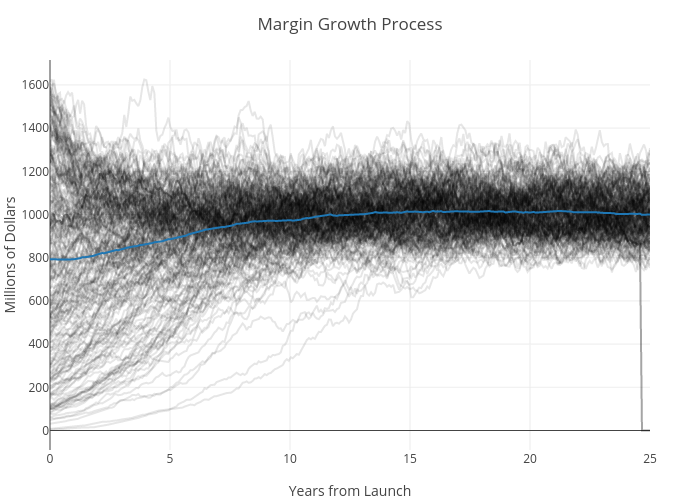
\includegraphics{./TaxationPlanImages/StochasticMarginGrowth.png}}
    \label{fig:sm_stochastic_margin_growth}
  \end{figure}
\end{center}

We first illustrate how the buybacks vary by the current level of margin. Note that this is very
similar to what we observed in the deterministic case --- At low levels of margin, we can support
a policy of zero buybacks because there is positive probability that the margin will grow to a point
where there will be relatively large buybacks. In the image below, we annualize the monthly buybacks
as a percent of margin

\begin{center}
  \begin{figure}[H]
    \scalebox{0.65}{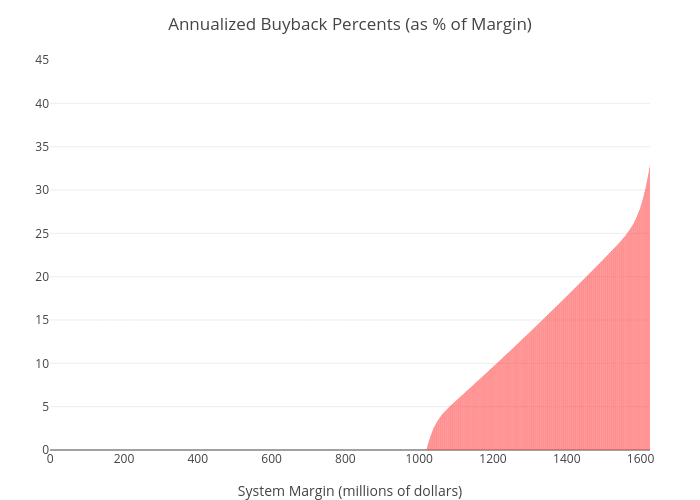
\includegraphics{./TaxationPlanImages/AnnualizedBuybacks.png}}
    \label{fig:sm_buybacks}
  \end{figure}
\end{center}

We now demonstrate how fees vary by the status of the rainy day fund and the current margin using
a heatmap. Current margin increases along the y-axis, the rainy day fund increases along the x-axis,
and the color of the image at a point demonstrates how high the annualized fee rates are at that
point.

\begin{center}
  \begin{figure}[H]
    \scalebox{0.65}{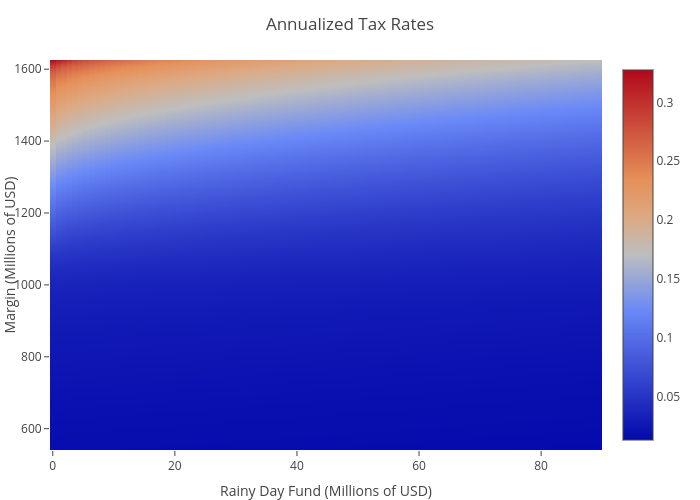
\includegraphics{./TaxationPlanImages/AnnualizedTaxRates.png}}
    \label{fig:sm_annualized_taxrates}
  \end{figure}
\end{center}

Finally, we simluated the entire system one time for 25 years. We plot each of the series of
interest below. We note that the fee rates are quite smooth relative to the buyback rates or the
amount held in the rainy day fund --- We view this as an indicator that the solution to our
mathematical program was a success.

\begin{center}
  \begin{figure}[H]
    \scalebox{0.45}{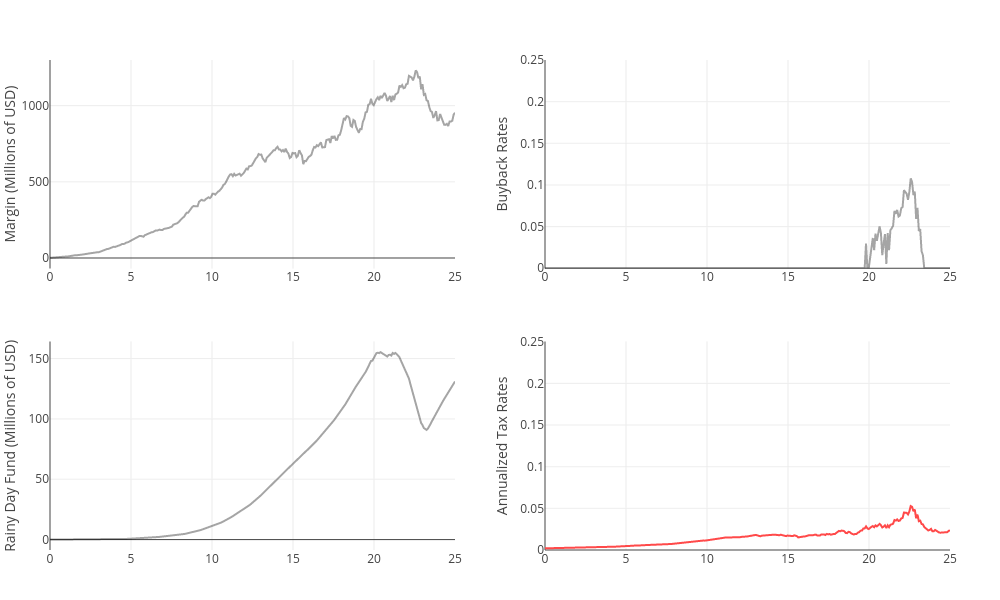
\includegraphics{./TaxationPlanImages/SimulationPlots.png}}
    \label{fig:sm_simulationplots}
  \end{figure}
\end{center}

\textbf{Tax Insights}

In this subsection, we discuss some of the findings associated with our numerical examples:

\vspace{0.25cm}

\textit{If there are no rainy day funds, fees must reflect at least the full buyback amount}

This point follows almost immediately from the fact that we have chosen to disallow any borrowing by
the DVM. If the rainy day fund, $D_t$, is currently at 0 then

\begin{align*}
  D_{t+1} + X_{t} \leq (1 + r)*D_t + F_t \\
  D_{t+1} + X_{t} \leq F_t
\end{align*}

The question is whether we will raise extra fees to not experience the same state tomorrow. It
turns out that if the margin is relatively low then we impose a slightly higher fee than needed to
provide additional stability for times in which we will have higher buybacks.

\vspace{0.25cm}

\textit{Rainy day funds are saved until periods when the buybacks are high}

This point is aimed at exploring $\frac{\partial X^*(M_t) - T^*(D_t, M_t)}{\partial M_t}$ and
$\frac{\partial X^*(M_t) - T^*(D_t, M_t)}{\partial D_t}$. It says, conditional on positive buybacks,
that the change in per-period savings is decreasing in both (1) how much savings there already is
and (2) the margin in the system.

\begin{align*}
  \frac{\partial (X^*(M_t) - T^*(D_t, M_t)) | X^*(M_t) > 0}{\partial D_t} &< 0 \\
  \frac{\partial (X^*(M_t) - T^*(D_t, M_t)) | X^*(M_t) > 0}{\partial M_t} &< 0
\end{align*}

\vspace{0.25cm}

\textit{Imposing low, but positive, fee rates while system is growing allows relatively low fee rates once margin is stable}

If we look at Figure ~\ref{fig:sm_simulationplots}, we can note that the annualized feerates are
approximately 0.2\% for the first 15 years and that during that time there are no buybacks. This
allows the system to build up its rainy day fund to almost 150 million USD. Shortly thereafter, the
system hits its maximum possible buyback levels which are approximately 10\% of the margin ---
Rather than impose extra high fee, it only raises the fee rates by a few percentage points and uses
the rainy day fund to fund the difference.
